\documentclass[10pt]{beamer}
\usepackage[utf8]{inputenc}
\usepackage[english]{babel}
\usepackage{alphabeta}
\usepackage{amsmath,amsthm,amsfonts,amssymb}
\usepackage{latexsym}
\usepackage[all,cmtip]{xy}
\usepackage{mathtools}
\usepackage{braket}
\usepackage[font=scriptsize,labelfont=bf]{caption}
\usepackage{tikz}
\usepackage{xmpmulti}
\usepackage{soul}

% set colors
\definecolor{myNewColorA}{RGB}{0, 109, 174}
\definecolor{myNewColorB}{RGB}{111, 100, 169}
\definecolor{myNewColorC}{RGB}{0, 111, 41}
\definecolor{myNewColorD}{RGB}{245, 123, 66}

\setbeamercolor*{titlelike}{fg=myNewColorA}
\setbeamercolor*{title}{bg=myNewColorA, fg = white}
\setbeamercolor*{caption name}{fg=myNewColorA}


% references
\usepackage{hyperref}

\newcommand*{\Scale}[2][4]{\scalebox{#1}{\ensuremath{#2}}}%
%------------------------------------------------------------

\setbeamerfont{title}{size=\large}
\setbeamerfont{subtitle}{size=\small}
\setbeamerfont{author}{size=\small}
\setbeamerfont{date}{size=\footnotesize}

\title{Faster than Hermitian time-evolution}
\subtitle{by Carl M Bender}
\author{Ana Fabela Hinojosa}
\institute[]{\includegraphics[scale=0.18]{logo.jpg}}
\date[\today]{Supervisors:\\ Jesper Levinsen\\ Meera Parish } 
%------------------------------------------------------------
% This block of commands puts the table of contents at the 
% beginning of each section and highlights the current section:
\AtBeginSection[]
{
 \begin{frame}
    \frametitle{Contents}
    \tableofcontents[currentsection]
 \end{frame}
}

% ------Contents below------
%------------------------------------------------------------

\begin{document}

%The next statement creates the title page.
\frame{\titlepage}
\begin{frame}
\frametitle{Outline}
\tableofcontents
\end{frame}

%------------------------------------------------------------

\section{Introduction}
\begin{frame}{Hilbert spaces}
\vspace{0.5cm}
A Hilbert space is a vector space that can be infinite dimensional. \\
\vspace{0.5cm}
Vector spaces are equipped with an inner product. \\
\vspace{0.5cm}
\textcolor{myNewColorD}{Inner product:\\
    Define a distance function.}
 \vspace{-1cm}
\begin{figure}
 \hspace{10em}
    \includegraphics[width=0.6\textwidth]{hilbert.pdf}
    \\
    \tiny{Fig.3: Hilbert space stuff}
    \end{figure}
\end{frame}


\begin{frame}{Hamiltonians as Observables}
    \centering{
    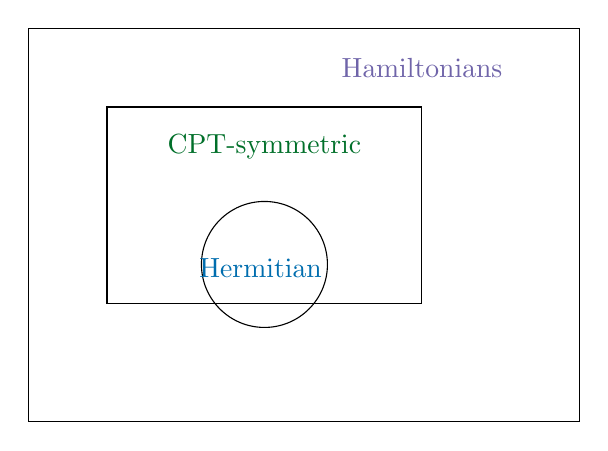
\begin{tikzpicture}
    \draw (-2,-1) rectangle(5,4) ++(-2,-0.5) node{\textcolor{myNewColorB}{Hamiltonians}};
    \draw (1,1) circle[x radius=0.8, y radius=0.8] ++(-0.05,-0.05) 
    node{\textcolor{myNewColorA}{Hermitian}};
    \pause
    \draw (-1,0.5) rectangle(3,3) ++(-2,-0.5) node{\textcolor{myNewColorC}{CPT-symmetric}};
    \end{tikzpicture}}
    \\
    \hspace{1em}
    \begin{tiny}
        Fig.1: The set of all possible Hamiltonians.
    \end{tiny}
    \\
    \begin{enumerate}
        \item \textcolor{myNewColorA}{Observables are \textbf{self-adjoint} operators $\{\hat{O}, \hat{H}, ...\}$}
        \item \textcolor{myNewColorC}{Real energy spectrum with defined lowest energy}
        \item \textcolor{myNewColorC}{A state $\psi$ of the quantum system is a unit vector of $\hat{H}$}
        \item \textcolor{myNewColorC}{Expectation values of observables are given by the inner-product.}
        \item \textcolor{myNewColorC}{Unitarity}
    \end{enumerate}
\end{frame}


\begin{frame}{Hamiltonians as Observables}
    \centering{
    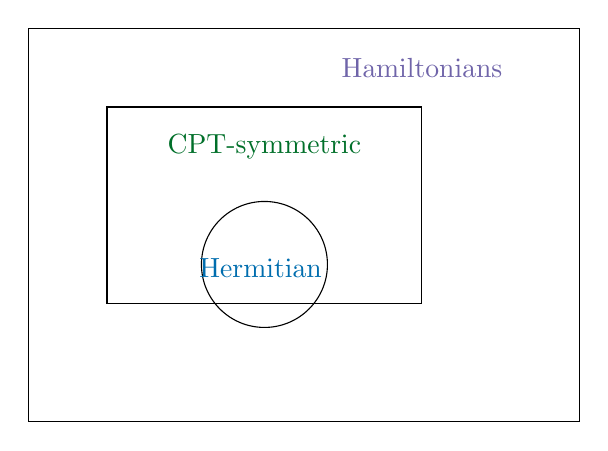
\begin{tikzpicture}
    \draw (-2,-1) rectangle(5,4) ++(-2,-0.5) node{\textcolor{myNewColorB}{Hamiltonians}};
    \draw (1,1) circle[x radius=0.8, y radius=0.8] ++(-0.05,-0.05) node{\textcolor{myNewColorA}{Hermitian}};
    \draw (-1,0.5) rectangle(3,3) ++(-2,-0.5) node{\textcolor{myNewColorC}{CPT-symmetric}};
    \end{tikzpicture}}
    \\
    \hspace{1em}
    \begin{tiny}
        Fig.1: The set of all possible Hamiltonians.
    \end{tiny}
    \\
    \begin{enumerate}
        \item \textcolor{myNewColorA}{\st{Observables are \textbf{self-adjoint} operators $\{\hat{O}, \hat{H}, ...\}$}}
        \item \textcolor{myNewColorC}{Real energy spectrum with defined lowest energy}
        \item \textcolor{myNewColorC}{A state $\psi$ of the quantum system is a unit vector of $\hat{H}$}
        \item \textcolor{myNewColorC}{Expectation values of observables are given by the inner-product.}
        \item \textcolor{myNewColorC}{Unitarity}
    \end{enumerate}
\end{frame}


\begin{frame}{CPT - symmetry in short}
    \vspace{-1cm}
    Hilbert space $\rightarrow \hat{H} = \hat{H}^{\mathcal{CPT}}$ \\
    \vspace{-0.4cm}
    \begin{align*}
        & \mathcal{C} \rightarrow \mathrm{charge\:conjugation},\\
        & \mathcal{P} \rightarrow \mathrm{spatial\:inversion},\\
        & \mathcal{T} \rightarrow \mathrm{complex\:conjugation\:and\:time\:reversal}.
    \end{align*}\\
    \vspace{0.5cm}
    Inner product is determined dynamically in terms of the Hamiltonian.\\
    \pause
    \vspace{0.5cm}
    If the eigenfunctions of a $\mathcal{PT}$-symmetric Hamiltonian are \textbf{not} also eigenfunctions of the $\mathcal{PT}$ operator we say the Hamiltonian possesess \textbf{broken $\mathcal{PT}$-symmetry}.\\
    \pause
    \vspace{0.5cm}
    Interesting physical phenomena occurs in the broken symmetry region
\end{frame}


\section{Time evolution}
\begin{frame}{Time evolution}
\vspace{-1cm}
\hspace{-2em}
\vspace{2cm}
\begin{columns}[T]
    \begin{column}{0.3\textwidth}
    \vspace{-2cm}
    \begin{align*}
    &\Scale[2]{\vec{\psi_{i}} \rightarrow{} \vec{\psi_{f}}}
    \end{align*}
    \pause
    \hspace{6em}
    \Scale[2.2]{\hookrightarrow}
    \end{column}
    
    \begin{column}{0.8\textwidth}
    \vspace{-1.3cm}
    \Scale[3]{\vec{\psi_{f}} = \hat{U} \vec{\psi_{i}}}\\
    \pause
    \hspace{6.8em}
    \begin{huge}
    {$\downarrow$}\\
    \end{huge}
    \begin{enumerate}
    \item \textcolor{myNewColorA}{Hermitian} quantum mechanics:\\
    \hspace{5em}
    $\hat{U} = e^{-i\hat{H}t / \hbar}$,\\
    \hspace{5em}
    where $t > 0$.
    \vspace{0.3cm}
    \pause
    \item \textcolor{myNewColorC}{CPT} quantum mechanics: \textcolor{myNewColorC}{\large{?}}
    \end{enumerate}
    \end{column}
    \end{columns}
\end{frame}


\section{Brachistochrone problem}
\begin{frame}{The Classical Brachistochrone problem}
\vspace{0.5cm}
\begin{columns}
    \hspace{1.5em}
    \begin{column}{\textwidth}
    \multiinclude[format=pdf,start=1,graphics={width=0.5\textwidth}]
    {optim-gif/optimisation}
    \\
    \hspace{1em}
    \tiny{Fig.2:
    A particle travels from left to right in time t,\\
    \hspace{2.4em}
    Can we make this trip nearly instantaneous?}
    \end{column}
    
    \hspace{-15em}
    \begin{column}{0.5\textwidth}
        βράχιστος χρόνος\\
        brákhistos khrónos:\\
        ``shortest time"\\
    \vspace{1cm}
    \pause
    \small{\textcolor{myNewColorC}{How fast can we evolve a state?}
    }
    \end{column}
    \end{columns}
\end{frame}


\begin{frame}{A simple quantum brachistochrone problem}
\begin{columns}
    \hspace{1.5em}
    \begin{column}{\textwidth}
    \includegraphics[width=0.35\textwidth]{bloch.png}\\
    \tiny{Fig.3: Bloch sphere with initial and final states}
    \end{column}
    \begin{column}{0.8\textwidth}
    \hspace{-20em}
    This space is spanned by $\vec{\psi_i}$ and $\vec{\psi_f}.$\\
    \vspace{0.4cm}
    \hspace{-20em}
    \pause
    We want the \textbf{fastest} time evolution possible,\\
    \hspace{-20em}
    without violating the time-energy uncertainty principle.\\
    \vspace{0.4cm}
    \pause
    \hspace{-20em}
    The chosen Hamiltonian must satisfy:\\
    \hspace{-20em}
    \textcolor{myNewColorD}{Energy constraint:}\\
    \hspace{-20em}
    \textcolor{myNewColorD}{$\quad\omega  = E_{\mathrm{max}} - E_{\mathrm{min}}$}\\
    \vspace{0.7cm}
    \pause
    \hspace{-18em}
    \textcolor{myNewColorC}{Will a complex non-Hermitian Hamiltonian}\\
    \hspace{-18em}
    \textcolor{myNewColorC}{give time-optimal evolution?}
    \end{column}
    \end{columns}
\end{frame}


\begin{frame}{The Maths}
\vspace{-1cm}
\begin{equation*}
    \vec{\psi_{i}}  = \begin{pmatrix}
                        1 \\
                        0 \\                
    \end{pmatrix}, \quad
    \vec{\psi_{f}}  = \begin{pmatrix}
                        a \\
                        b \\                
    \end{pmatrix}
    = \begin{pmatrix}
                        0 \\
                        1 \\                
    \end{pmatrix}
    \vspace{0.5cm}
    \end{equation*}. \\

    \begin{columns}
    \begin{column}{0.5\textwidth}
    \textcolor{myNewColorA}{Hermitian} case
    \hspace{-3em}
    \begin{scriptsize}
    \begin{equation*}
    \hat{H}  = \begin{pmatrix}
                s & r e^{-i\theta}  \\
                r e^{i \theta} & u  \\
                \end{pmatrix} , \{r, s, \theta, u\} \in \mathbb{R},
    \end{equation*}\\
    \textcolor{myNewColorD}{Energy constraint}
    \hspace{-1.5em}
    \begin{equation*}
        \textcolor{myNewColorD}{\omega^2 = (s-u)^2 + 4r^2},
    \end{equation*}\\

    Time evolution
    \hspace{-1.5em}
    \begin{equation*}
        \begin{pmatrix}
            a \\
            b \\                
            \end{pmatrix} = e^{\frac{-i(s+u)t}{2\hbar}}\begin{pmatrix}
            \cos(\frac{\omega t}{2\hbar}) - i \frac{s - u}{\omega} \sin(\frac{\omega t}{2\hbar})\\
            - i \frac{2r}{\omega} e^{i \theta} \sin(\frac{\omega t}{2\hbar}) \\
            \end{pmatrix}.
    \end{equation*}\\
    \end{scriptsize}
    \end{column}

    \begin{column}{0.5\textwidth}
    \textcolor{myNewColorC}{CPT-symmetric} case
    \begin{scriptsize}
    \begin{equation*}
    \Tilde{H}  = \begin{pmatrix}
                r e^{i\theta} & s  \\
                s & r e^{-i\theta}  \\
                \end{pmatrix}, \quad \{r, s, \theta\} \in \mathbb{R},
    \end{equation*}\\
    \textcolor{myNewColorD}{Energy constraint}
    \hspace{-1.5em}
   \begin{equation*}
        \textcolor{myNewColorD}{\omega^2 = 4s^2 - 4r^2 \sin^2{\theta}} > 0,
    \end{equation*}\\
    Time evolution
    \hspace{-1.5em}
    \begin{equation*}
        \begin{pmatrix}
                a \\
                b \\                
        \end{pmatrix} = \frac{e^{\frac{-itr \cos\theta}{\hbar}}}{\cos{\alpha}}
        \begin{pmatrix}
                \cos(\frac{\omega t}{2 \hbar} - \alpha)\\
                - i \sin(\frac{\omega t}{2\hbar})\\
        \end{pmatrix}.
    \end{equation*}\\
    \hspace{-1.5em}
    where $\sin(\alpha) = \frac{r}{s}\sin(\theta)$.

    \end{scriptsize}
    \end{column}
\end{columns}
\end{frame}


\begin{frame}{The Maths}
\begin{scriptsize}
\begin{equation*}
    \vec{\psi_{i}}  = \begin{pmatrix}
                        1 \\
                        0 \\                
    \end{pmatrix}, \quad
    \vec{\psi_{f}}  = \begin{pmatrix}
                        a \\
                        b \\                
    \end{pmatrix}
    = \begin{pmatrix}
                        0 \\
                        1 \\                
    \end{pmatrix}
    \end{equation*}\\
    \end{scriptsize}
    \vspace{0.3cm}

    \begin{columns}
    \begin{column}{0.5\textwidth}
    \textcolor{myNewColorA}{Hermitian} time evolution\\

    \begin{scriptsize}
    \begin{equation*}
        \begin{pmatrix}
            a \\
            b \\                
            \end{pmatrix} = e^{\frac{-i(s+u)t}{2\hbar}}\begin{pmatrix}
            \cos(\frac{\omega t}{2\hbar}) - i \frac{s - u}{\omega} \sin(\frac{\omega t}{2\hbar})\\
            - i \frac{2r}{\omega} e^{i \theta} \sin(\frac{\omega t}{2\hbar}) \\
            \end{pmatrix}.
    \end{equation*}
    \pause
    \begin{equation*}
    \Rightarrow |b|= \frac{2r}{\omega} \sin\left(\frac{\omega t}{2\hbar}\right),
    \end{equation*}
    \pause
    \begin{equation*}
    \Rightarrow t = \frac{2\hbar}{\omega} \arcsin\left(\frac{\omega |b|}{2r}\right),
    \end{equation*}
    \pause
    For all $r>0$ subject to \textcolor{myNewColorD}{$\omega^2 = (s-u)^2 + 4r^2$}\\
    for a fixed $\omega$.
    \begin{equation*}
    \therefore \tau = \frac{2\hbar}{\omega} \arcsin\left(|b|\right) = \frac{\pi \hbar}{\omega}
    \end{equation*}\\
    is the minimum \textit{passage time}.
    \end{scriptsize}
    \end{column}

    \pause
    \begin{column}{0.5\textwidth}
    \vspace{2cm}
    \textcolor{myNewColorC}{CPT} time evolution\\
    \vspace{-1cm}
    \begin{scriptsize}
    \begin{equation*}
        \begin{pmatrix}
                a \\
                b \\                
        \end{pmatrix} = \frac{e^{\frac{-itr \cos\theta}{\hbar}}}{\cos{\alpha}}
        \begin{pmatrix}
                \cos(\frac{\omega t}{2 \hbar} - \alpha)\\
                - i \sin(\frac{\omega t}{2\hbar})\\
        \end{pmatrix}.
    \end{equation*}\\
    \pause
    \begin{equation*}
    \Rightarrow |a|= \frac{\cos{\frac{\omega t}{2 \hbar} -\alpha}}{\cos{\alpha}} \sin\left(\frac{\omega t}{2\hbar}\right),
    \end{equation*}
    \pause
    \begin{equation*}
    \Rightarrow t = \frac{\hbar}{\omega}(2 \alpha + \pi) ,
    \end{equation*}
    \pause
    Since $\omega$ is fixed,
    \textcolor{myNewColorD}{$\omega^2 = 4s^2 - 4r^2 \sin^{2}(\theta)$}\\
    $\quad\quad\quad\quad\:\:\:\quad \to \omega^2 = 4s^2\cos^2(\alpha)$\\
    we require $s, r >> 1$.\\
    \pause
    \vspace{0.5cm}
    Then $t \to 0$ when $\alpha \to -\frac{\pi}{2}$.\\
    \end{scriptsize}
    \end{column}
\end{columns}
\end{frame}


\begin{frame}{The geometry of the space}
\begin{columns}
    \hspace{1.5em}
    \begin{column}{\textwidth}
    $\mathcal{CPT}$ inner products are defined depending on the Hamiltonian used.\\
    \pause
    \vspace{0.5cm}
    \begin{equation*}
        \vec{\psi_i} = \begin{pmatrix}
                1 \\
                0 \\                
        \end{pmatrix}, \quad
        \vec{\psi_f} = \begin{pmatrix}
                0 \\
                1 \\                
        \end{pmatrix}
        \end{equation*}
    \begin{enumerate}
        \item orthogonal $\to$ \textcolor{myNewColorA}{Hermitian} inner product
        \pause
        \item not orthogonal $\to$ \textcolor{myNewColorC}{CPT}  inner  product\\
        \pause
        vector separation: $\delta = \pi - 2|\alpha|$\\
        \pause 
        \vspace{0.5cm}
        We can choose $\alpha$ to create a ``wormhole" effect in Hilbert space.
        \end{enumerate}
    \end{column}
\end{columns}
\end{frame}

\section{Conclusion}
\begin{frame}{Conclusion}
\begin{enumerate}
    \item This paper demonstrates the theoretical differences in both $\mathcal{PT}$-symmetric and conventional Hermitian quantum mechanics.\\
    \item The ``wormhole" effect could be of importance in design and implementation of fast quantum computation and comunication algorithms.\\
    \item There could be quantum protection mechanisms limiting the applicability of Hilbert-space ``wormholes".
\end{enumerate}
\end{frame}

\begin{frame}{References} 
    \nocite{*}
    \bibliographystyle{unsrturl_mod}
    \bibliography{mybib.bib}
\end{frame}

% \section{Appendix}
% \begin{frame}{Broken and unbroken CPT-symmetry}
% \end{frame}

% \begin{frame}{Constructing the C operator}
% \begin{equation*}
% \mathcal{C}^2 = 1,\quad [\mathcal{C}, \hat{H}] = 0,\quad [\mathcal{C},\mathcal{PT}] = 0.
% \end{equation*}

% \end{frame}

% \begin{frame}{Equivalent Hermitian and PT symmetic Hamiltonians}
% For any Hamiltonian with unbroken $\mathcal{PT}$-symmetry there exists an equivalent Hermitian Hamiltonian.
% \begin{enumerate}
%     \item
% \end{enumerate}
% \end{frame}

% \begin{frame}{More CPT quantum theory}
% \begin{columns}
%     \hspace{1.5em}
%     \begin{column}{\textwidth}
%     \begin{enumerate}
%     \item \begin{large}Balanced open systems\\
%     \end{large}
%         \vspace{0.1cm}
%         \begin{small}
%         Imaginary potential contributions $\rightarrow$ source and drain terms.
%         \end{small}

%     \item \begin{large}Possible experimental ideas\\
%     \end{large}
%     \vspace{0.1cm}
%     \begin{small}Embedding the non-Hermitian CPT symmetric system into a larger structure described by a Hermitian Hamiltonian.
%     \end{small}
%     \end{enumerate}
%     \end{column}
% \end{columns}
% \end{frame}

% \begin{frame}{Rabi frequency}
% \begin{columns}
%     \hspace{1.5em}
%     \begin{column}{\textwidth}
%     The frequency of fluctuations in the populations of two atomic energy levels.\\
%     \vspace{0.5cm}
%     It is proportional to the strength of the \textbf{coupling} between the light's and the atomic transition's frequencies. 
%     \end{column}
% \end{columns}
% \end{frame}

\end{document}





